\documentclass[12pt, letterpaper] {article}

\parindent=5mm
\usepackage[spanish]{babel}

\usepackage{amssymb}
\usepackage{amsmath} 
\usepackage{amsfonts}

\usepackage[numbers,sort&compress]{natbib}
\usepackage{graphicx}

\usepackage{url}
\usepackage{hyperref}

\usepackage[top=25mm, bottom=20mm, left=1.5cm, right=1.5cm]{geometry}
\setlength{\parskip}{2mm}
\setlength{\parindent}{1pt}

\usepackage{listings}

\usepackage{float}

\usepackage[utf8]{inputenc}
\usepackage{graphicx} 
\usepackage{subfigure} 

\usepackage{color}
\usepackage{multirow}

\definecolor{dkgreen}{rgb}{0,0.6,0}
\definecolor{gray}{rgb}{0.5,0.5,0.5}
\definecolor{mauve}{rgb}{0.58,0,0.82}

\usepackage{color}
\usepackage{listings}
\lstset{ %
  language=R,                     % the language of the code
  basicstyle=\footnotesize,       % the size of the fonts that are used for the code
  numbers=left,                   % where to put the line-numbers
  numberstyle=\tiny\color{gray},  % the style that is used for the line-numbers
  stepnumber=1,                   % the step between two line-numbers. If it's 1, each line
                                  % will be numbered
  numbersep=5pt,                  % how far the line-numbers are from the code
  backgroundcolor=\color{white},  % choose the background color. You must add \usepackage{color}
  showspaces=false,               % show spaces adding particular underscores
  showstringspaces=false,         % underline spaces within strings
  showtabs=false,                 % show tabs within strings adding particular underscores
  frame=single,                   % adds a frame around the code
  rulecolor=\color{black},        % if not set, the frame-color may be changed on line-breaks within not-black text (e.g. commens (green here))
  tabsize=2,                      % sets default tabsize to 2 spaces
  captionpos=b,                   % sets the caption-position to bottom
  breaklines=true,                % sets automatic line breaking
  breakatwhitespace=false,        % sets if automatic breaks should only happen at whitespace
  title=\lstname,                 % show the filename of files included with \lstinputlisting;
                                  % also try caption instead of title
  keywordstyle=\color{blue},      % keyword style
  commentstyle=\color{dkgreen},   % comment style
  stringstyle=\color{mauve},      % string literal style
  escapeinside={\%*}{*)},         % if you want to add a comment within your code
  morekeywords={*,...}            % if you want to add more keywords to the set
} 


\author{Ricardo Rosas Macías \\[0.9mm] Universidad Autónoma de Nuevo León}

\title{Propuesta de método de agitación mecánica asistido con ultrasonido para desaglomeración de nanopartículas}


\date{\today}

\begin{document}


\twocolumn[
\begin{@twocolumnfalse}

\maketitle

\begin{center}\rule{0.9\textwidth}{0.1mm} \end{center}
\begin{abstract}

\normalsize 
Este trabajo muestra una solución para la aglomeración de nanopartículas, puesto que los estudios existentes señalan que las principales características de las nanopartículas dispersas tienen una estrecha relación con sus propiedades superficiales; en atención a lo cual proporcionan otras propiedades que no se muestran en bulk y micro escala. Asimismo, se presentan las condiciones de experimentación de la simulación en el software $R$, así como su análisis estadístico, que permiten evidenciar el comportamiento esperado por la propuesta inicial.\\ \\
Palabras clave: Aglomeración, Nanopartículas, Simulación, Software $R$.
\begin{center}\rule{0.9\textwidth}{0.1mm} \end{center}
\end{abstract}

\end{@twocolumnfalse} 
]

\section{Introducción}

Las nanopartículas contienen solo unos pocos átomos, a diferencia de los materiales en bulk (bulto), que podrían contener muchos miles de millones de átomos. Esta diferencia es lo que hace que los nano polvos se comporten de manera diferente a sus contrapartes en masa \cite{RINyN}. Se reconoce que, cuando el tamaño de una partícula disminuye a nanoescala, las propiedades físicas y químicas de la partícula cambiarán; esto significa que las partículas de tamaño nanométrico, tienen propiedades ópticas, eléctricas, mecánicas, magnéticas, entre otras, que difieren sustancialmente de las partículas más grandes del mismo elemento o compuestos del cual esta constituido \cite{BN}.

La superficie de una nanopartícula está hecha de átomos/moléculas que están menos ligadas a las partículas que las del bulto. Cuanto más pequeña es la partícula, mayor es el debilitamiento del enlace. El debilitamiento de la unión se distribuye a lo largo de un diámetro de la partícula en un número finito de capas, este número depende del material. Por lo tanto, los átomos/moléculas de partículas pequeñas se disuelven más fácilmente que los de partículas grandes, mientras que los átomos/moléculas están más fuertemente unidos a partículas grandes. Por consiguiente, se forma un cluster a causa del intercambio de materia que va de las partículas pequeñas a las más grandes \cite{BNNP}. 

Los clusters son un conjunto de nanopartículas primarias aglomeradas; unidas entre sí en las esquinas o bordes, de manera que no son unidades fijas, por lo cual pueden cambiar su tamaño y forma, dependiendo del conjunto de partículas con las que este constituido. Por esta razón, la densidad de los clusters depende de la distribución del tamaño de las partículas primarias aglomeradas; de acuerdo a su geometría y composición química. 

Esta aglomeración se debe principalmente a la alta energía superficial que tiene este tipo de nanopartículas, por lo que tienden a aglomerarse para disminuir esta energía. A medida que estas se encuentran guardadas en un recipiente, sufren de un proceso de aglomeración a lo largo del tiempo, debido a las fuertes interacciones de de Van der Waals, que permite la formación de clusters; que posteriormente se vuelven más grandes por la interacción cluster-cluster. 

La aglomeración de nanopartículas es normalmente un proceso irreversible por el método de ultrasonido. La aplicación de ultrasonidos a los nanomateriales tiene múltiples efectos. Lo más común es la dispersión de nanopartículas en líquidos para romper los aglomerados, debido a las implociones de las microburbujas que genera, permiten realizar una fuerza que irrumpe la fuerza de Van der Waals que esta interactuando con las partículas que se encuentran aglomeradas, de manera que posteriormente, se obtienen partículas dispersas individuales. Esto hace que el ultrasonido sea un medio eficaz para la dispersión, además de su fácil aplicación y escalamiento; hasta un nivel industrial \cite{UDD}.

\section{Antecedentes}

En las industrias de tintas, pinturas y recubrimientos, la dispersión, desaglomeración y molienda en húmedo de pigmentos en polvo y nanopartículas es una aplicación básica con consecuencias fundamentales para la calidad del producto \cite{WUD}. 
La mayoría de los pigmentos son muy costosos, por lo tanto, el esfuerzo de la industria de fabricación de tinta se centra en la producción de tinta de alta calidad con la mayor resistencia de color y una menor cantidad posible de pigmento. Una dispersión más rápida y un aumento de la capacidad de producción ayudan a reducir los costos. El grado de uniformidad de las partículas y la uniformidad de la dispersión son esenciales para lograr un mayor brillo de la tinta, una mayor intensidad del color y una mejor apariencia. Debido a estos hechos, se necesita equipo confiable de alta potencia para el procesamiento de pigmentos \cite{UDNPS}. 

La dispersión ultrasónica ha sido probada en diferentes estudios por su eficiencia y confiabilidad en lo que respecta a su desempeño en tratamientos de pigmentos para la fabricación de tinta. Los requisitos que deben cumplir las dispersiones de pigmentos incluyen un tamaño de partícula inferior a 100 nm, estabilidad coloidal, compatibilidad de varios componentes de tinta y pureza \cite{UDINER} \cite{ODCNTUS}.

En términos de poder del ultrasonido, existen dos tipos de ultrasonidos usados comúnmente en el laboratorio: el ultrasonido de baño y de sonda \cite{UPSR}. El ultrasonido de baño tiene una potencia menor de usualmente menos de 100 W, mientras que el de sonda produce una potencia mayor, generalmente en el rango de 100–1500 W, con amplitud de potencia ajustable; de modo que este permite tener una mayor potencia y por consiguiente una mejor fuerza de separación de nanopartículas \cite{UDENAS}. En contraste, tanto el poder de sonicación como el tiempo son parámetros importantes para controlar, para una dispersión homogénea de nanopartículas \cite{NFDP} \cite{EUTNC}. 

\section{Propuesta}

Se plantea el uso de un sistema de agitación mecánica asistido con ultrasonido, para obtener una mejor distribución de aglomeración nanopartículas en el recipiente, por consiguiente se busca una homogeneización de tamaño de las nanopartículas. 

Este sistema cuenta con un ultrasonido de sonda con un mecanismo que permite la incorporación de una agitación mecánica en la sonda, como se observa en la figura \ref{MUSAG}, de manera que permite controlar la cinética y obtener mejores tamaños monodispersos.

\begin{figure}[H]
\centering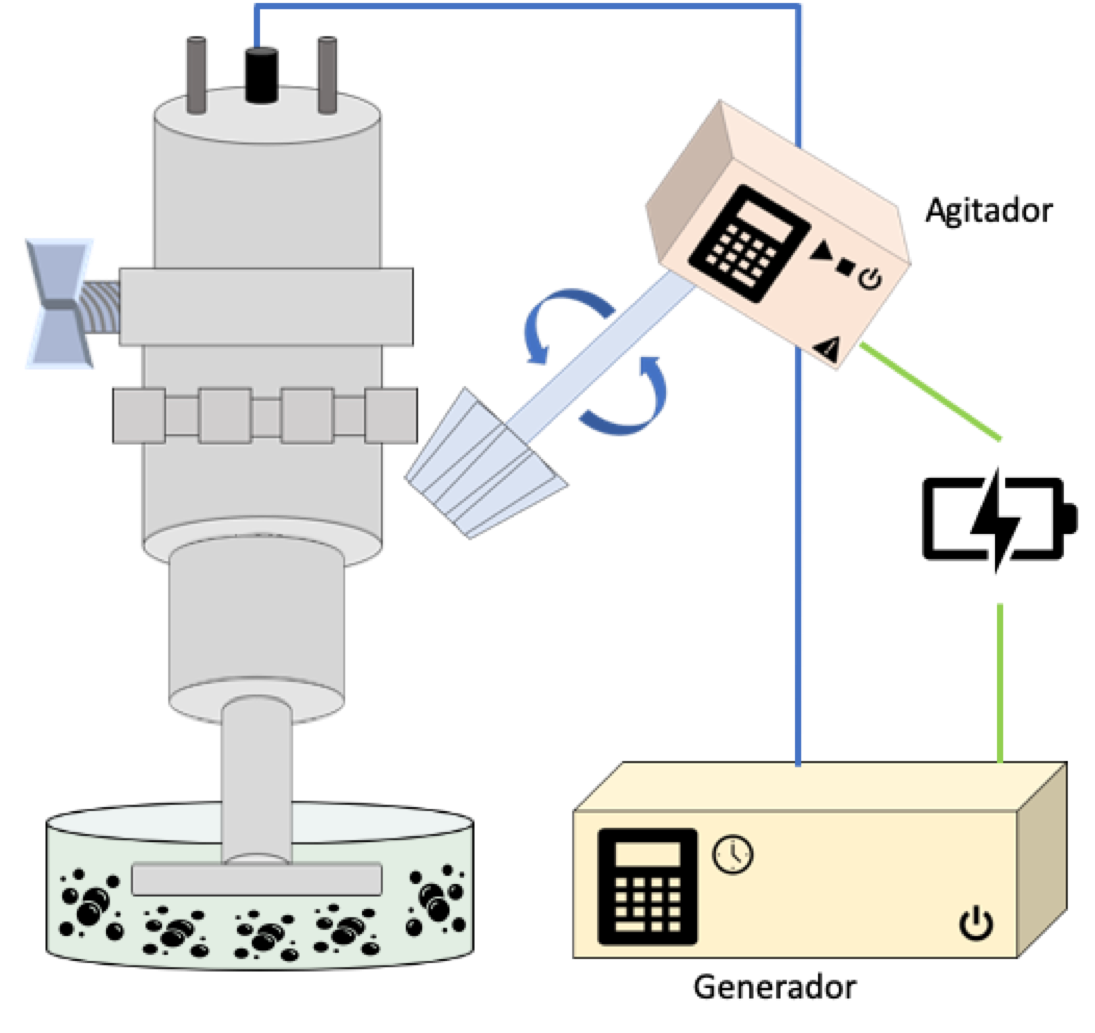
\includegraphics[width=82mm]{USconAg.png}
\caption{Representación del sistema de ultrasonido con agitación mecánica}
\label{MUSAG}
\end{figure}

\section{Objetivo}

La finalidad de la simulación es desarrollar un código que muestre el comportamiento del sistema propuesto, con una visualización en 2D. Asimismo, demostrar el efecto en el tamaño de las nanopartículas desaglomeradas. 

\section{Especificaciones de equipo}
 
Para llevar acabo la simulación del experimento, se uso una MacBook Pro Mid 2012 con el sistema operativo macOS Mojave 10.14.5, que cuenta con un procesador Intel Core i5 de 2.5 GHz, una memoria ram DDR3 de 8 GB de 1333 MHz, un disco SSD Kingston A400 de 480GB y una tarjeta gráfica Intel HD Graphics 4000 de 1536 MB.
 
 
\section{Metodología}
 
Para realizar el código, se tomo una referencia de acuerdo a la literatura anteriormente reportada \cite{elisawebIEP} \cite{MP9}. 

En las primeras líneas se muestra los parámetros iniciales del experimento; en donde se le asignó el área del recipiente (radio=$r$, coordenadas=$cx$,$cy$), así como área que le pertenece a la punta de la sonda del ultrasonido (radio=$ri$, coordenadas=$cix$,$ciy$).

\begin{lstlisting}[language=R]
r <- 30
ri <- 5
n <- 200 
circle <- seq(0,360,0.005)
cx <- r * cos(circle)
cy <- r * sin(circle)
cix <- ri * cos(circle)
ciy <- ri * sin(circle)
\end{lstlisting}

Se determinó los ángulos que tendrá el movimiento de las partículas ($theta$) y el radio de los clusters inicial ($rad$), también se decretó las coordenas cratesianas que tendrán las nanopartículas ($xp$, $yp$) y de la barra ($xl$, $yl$), así como la velocidad de la barra ($a$).
 
\begin{lstlisting}[language=R]
theta <- (pi*2) * runif(n)
rad <- runif(n,ri,r)
xp <- rad * cos(theta)
yp <- rad * sin(theta)
a <- seq(0,2*pi-0.00001,2*pi/360)
xl <- r * cos(a) 
yl <- r * sin(a) 
\end{lstlisting}

Se creo un Data Frame que permitiera guardar los parámetros de las nanopartículas, además se definió una densidad y un radio respecto a la masa de las partículas.

\begin{lstlisting}[language=R]
p <- data.frame(x= xp, y = yp, m=runif(n,10,60),radio = rad, angulo = atan2(yp,xp),vel = (2*pi)/sample(180:450,length(xp)))
dens<-0.5
p$ram<-sqrt(p$m/(dens*pi))/5 
\end{lstlisting}

Además se estableció un giro en los 360º del área del recipiente y se dibujaron las nanopartículas dentro de este espacio de agitación.

\begin{lstlisting}[language=R]
for(i in 1:360) { #Pasos de la barra por frame
  png(paste("MovPar_d", i,".png", sep=""))
  plot(1, type="n", xlab="", ylab="", xlim=c(-r,r),ylim=c(-r,r), main = paste("angulo: ", i, sep = '') )
  lines(cy~cx,col="red") #circulo exterior
  lines(ciy~cix) #circulo interior
  segments(rep(0,length(xp)),rep(0,length(yp)),xl[i],yl[i],col="blue") #Barra 0 grados
  segments(rep(0,length(xp)),rep(0,length(yp)),-xl[i],-yl[i],col="blue") #Barra 180 grados
  for(j in 1:length(p$x)) {
    draw.circle(p$x[j],p$y[j],p$ram[j],col="red") #Dibujado de particulas
  }
\end{lstlisting}

Como también se actualizaron las coordenadas de las nanopartículas respecto al movimiento (ángulo) generado por la agitación, de igual manera se añadió su velocidad angular.

\begin{lstlisting}[language=R]
  p$x <- p$radio * cos(p$angulo) 
  p$y <- p$radio * sin(p$angulo)
  p$angulo <- p$angulo + p$vel 
  graphics.off()
}
\end{lstlisting}

 
\section{Resultados}

Se logró obtener un gif que muestra el movimiento de las partículas generado por la agitación mecánica, se tomaron las imágenes más representativas, que se pueden observar en la figura \ref{MovP}

\begin{figure}[]
\centering
\subfigure[Giro de propela a 1º]{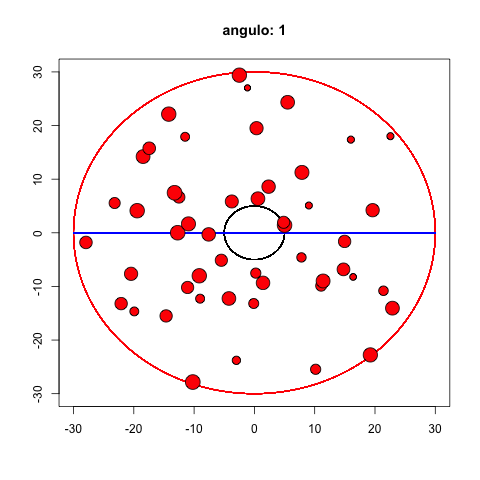
\includegraphics[width=44mm]{./MovPar_d1}}\vspace{1mm}
\subfigure[Giro de propela a 90º]{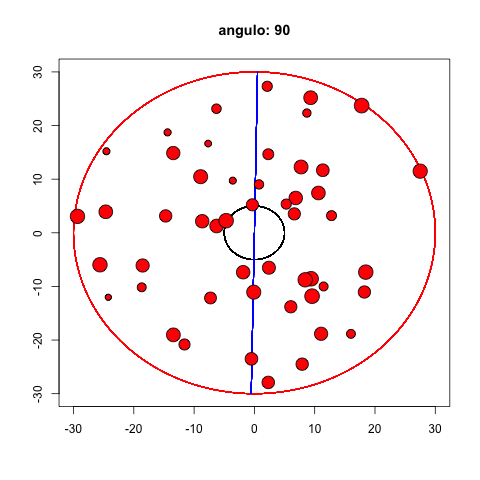
\includegraphics[width=44mm]{./MovPar_d90}}
\subfigure[Giro de propela a 270º]{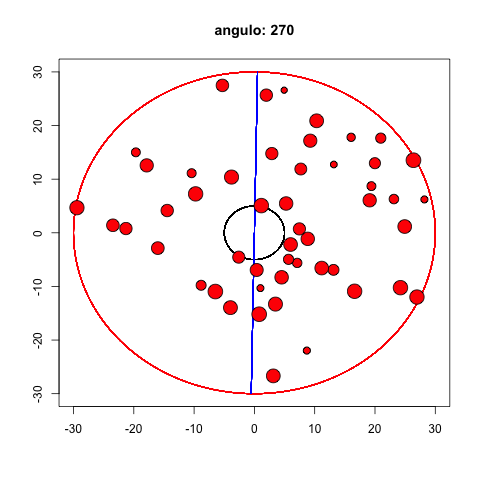
\includegraphics[width=44mm]{./MovPar_d270}}\vspace{1mm}
\subfigure[Giro de propela a 360º]{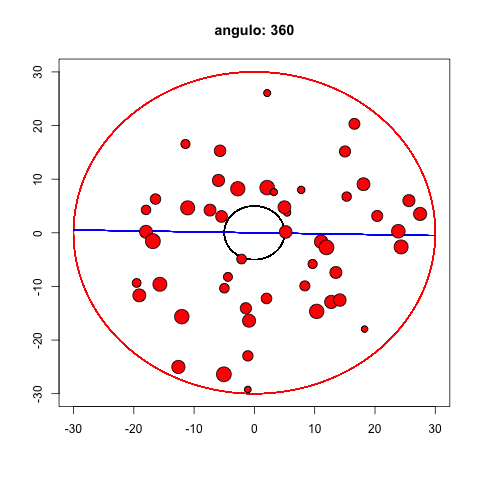
\includegraphics[width=44mm]{./MovPar_d360}}
\caption{Mezcla de nanopartículas}\label{MovP}
\end{figure}

\subsection{Discusión}

En la figura \ref{MovP} claramente evidencia el movimiento de una agitación de los clusters, pero no se puede apreciar la desaglomeración por parte del ultrasonido.

\section{Conclusiones}

La simulación no tuvo éxito para concluir con su objetivo, por lo cual se recomienda seguir añadiendo parámetros que permitan conocer la naturaleza del experimento.


\section{Trabajo a futuro}

Este sistema cuenta con una gran aplicación, por lo cual se puede agregar más parámetros que permitan determinar las condiciones mejor detalladas para encontrar el tiempo efectivo de desaglomeración a diferentes frecuencias. Asimismo se puede realizar un diseño de una mejor propela para un generar un flujo óptimo de las nanopartículas en la solución. De manera que, la simulación permitirá conocer el funcionamiento teórico del sistema, así en futuro esto permitirá comparar la teoría con la practica e incluso si se obtienen buenos resultados, se podrá escalar el proceso.

\section{Agradecimientos}

Me gustaría agradecer a la Dra. Satu Elisa Schaeffer por su asesoría, para la elaboración de este proyecto. Como también, a mis compañeros Edson Cepeda Márquez y Marco Guajardo Vigil por su apoyo. 

\bibliographystyle{plainnat}

\bibliography{BiblioFProject}

\end{document}